\documentclass[12pt, twoside]{article}
\usepackage[letterpaper, margin=1in, headsep=0.5in]{geometry}
\usepackage[english]{babel}
\usepackage[utf8]{inputenc}
\usepackage{amsmath}
\usepackage{amsfonts}
\usepackage{amssymb}
\usepackage{tikz}
%\usetikzlibrary{quotes, angles}

\usepackage{graphicx}
\usepackage{enumitem}
\usepackage{multicol}

\usepackage{fancyhdr}
\pagestyle{fancy}
\fancyhf{}
\renewcommand{\headrulewidth}{0pt} % disable the underline of the header

\fancyhead[LE]{\thepage}
\fancyhead[RO]{\thepage \\ Name: \hspace{4cm} \,\\}
\fancyhead[LO]{BECA / Dr. Huson / Geometry\\* Unit 6: Distance \& slope\\* 5 December 2019}

\begin{document}
\subsubsection*{6.7 Classwork: Midpoint graphs and the midpoint formula}
  \begin{enumerate}

  \item Given $\overleftrightarrow{AB}$ as shown on the number line, with $A=-3$ and $B=5$. Mark and label the midpoint $M$ between $A$ and $B$?\\[20pt] % Midpoint
  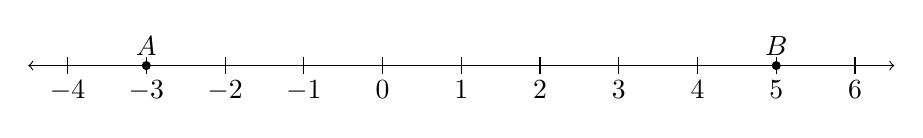
\begin{tikzpicture}
    \draw [<->] (-4.5,0)--(6.5,0);
    \foreach \x in {-4,...,6} %2 leading for diff!=1
      \draw[shift={(\x,0)},color=black] (0pt,-3pt) -- (0pt,3pt) node[below=5pt]  {$\x$};
      \draw [fill] (-3,0) circle [radius=0.05] node[above] {$A$};
      \draw [fill] (5,0) circle [radius=0.05] node[above] {$B$};
  \end{tikzpicture}
  
  \item On the graph below, draw $\overline{AB}$, with $A(2,3)$ and $B(8,3)$, labeling the end points. Determine and state the coordinates of the midpoint $M$ of $\overline{AB}$ and mark and label it on the graph.
  \begin{flushright}
    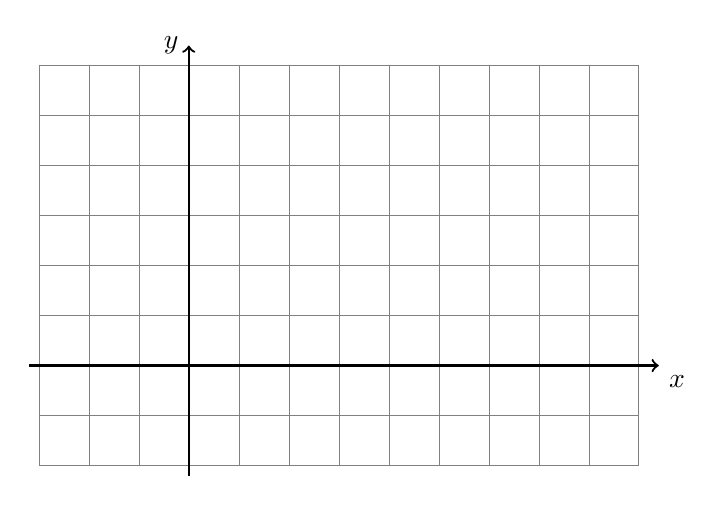
\begin{tikzpicture}[scale=.635]
      \draw [help lines] (-3,-2) grid (9,6);
      \draw [thick, ->] (-3.2,0) -- (9.4,0) node [below right] {$x$};
      \draw [thick, ->] (0,-2.2)--(0,6.4) node [left] {$y$};
    \end{tikzpicture}
  \end{flushright}
  
  
  \item On the graph below, draw $\overline{AB}$, with $A(1,2)$ and $B(7,4)$, labeling the end points. Determine and state the coordinates of the midpoint $M$ of $\overline{AB}$ and mark and label it on the graph.
  \begin{flushright}
    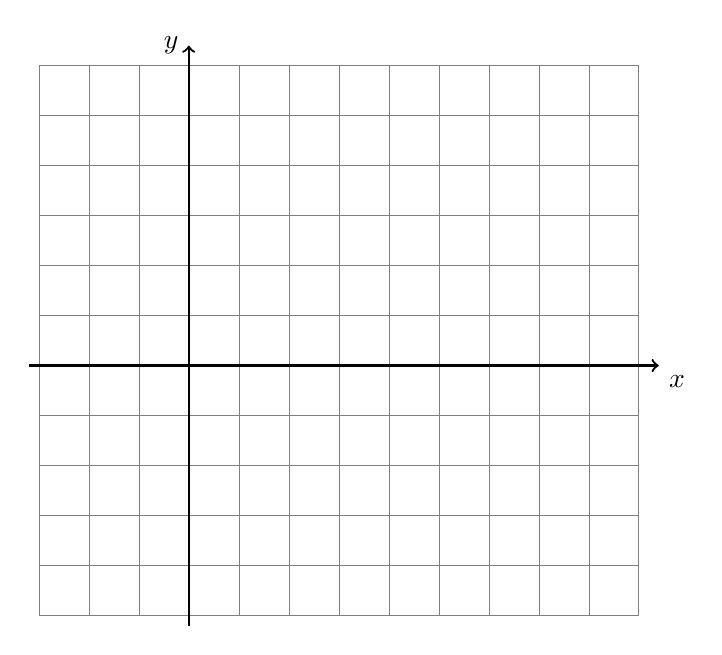
\begin{tikzpicture}[scale=.635]
      \draw [help lines] (-3,-5) grid (9,6);
      \draw [thick, ->] (-3.2,0) -- (9.4,0) node [below right] {$x$};
      \draw [thick, ->] (0,-5.2)--(0,6.4) node [left] {$y$};
    \end{tikzpicture}
  \end{flushright}
  \vspace{1cm}

\newpage
  \item On the graph below, draw $\overline{AB}$, with $A(-1,3)$ and $B(5,1)$, labeling the end points. Determine and state the coordinates of the midpoint $M$ of $\overline{AB}$ and mark and label it on the graph.
  \begin{flushright}
    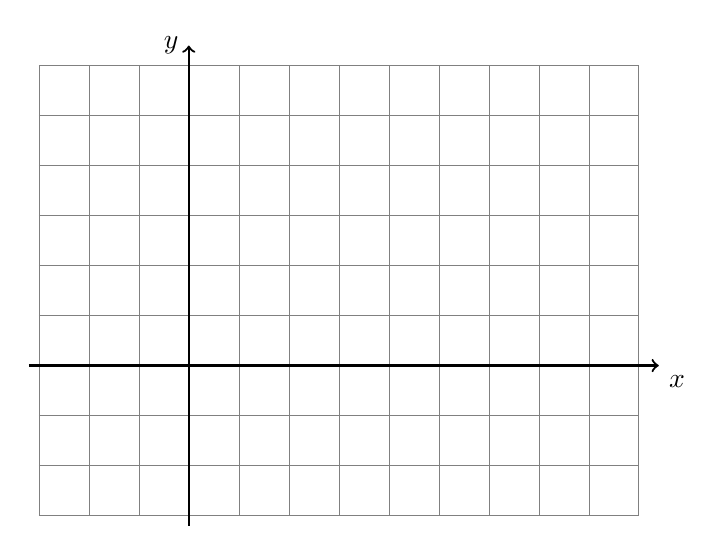
\begin{tikzpicture}[scale=.635]
      \draw [help lines] (-3,-3) grid (9,6);
      \draw [thick, ->] (-3.2,0) -- (9.4,0) node [below right] {$x$};
      \draw [thick, ->] (0,-3.2)--(0,6.4) node [left] {$y$};
    \end{tikzpicture}
  \end{flushright}

  \item On the graph below, draw $\overline{AB}$, with $A(3,-3)$ and $B(7,5)$, labeling the end points. Determine and state the coordinates of the midpoint $M$ of $\overline{AB}$ and mark and label it on the graph.
  \begin{flushright}
    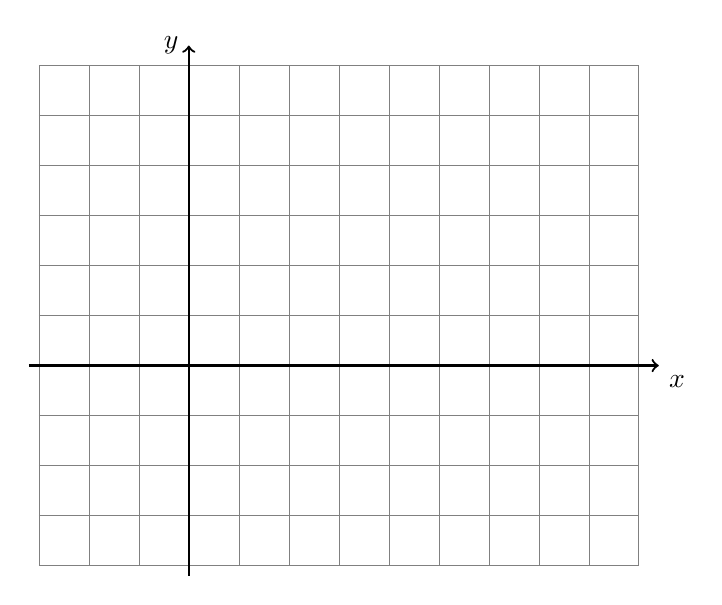
\begin{tikzpicture}[scale=.635]
      \draw [help lines] (-3,-4) grid (9,6);
      \draw [thick, ->] (-3.2,0) -- (9.4,0) node [below right] {$x$};
      \draw [thick, ->] (0,-4.2)--(0,6.4) node [left] {$y$};
    \end{tikzpicture}
  \end{flushright}

\item Use the midpoint formula to find the midpoint of $A(4,10)$, $B(12,2)$.

\end{enumerate}
\end{document}

